\documentclass[]{report}

\usepackage[square, numbers]{natbib}
\usepackage{graphicx}
\usepackage{caption}
\usepackage{subcaption}
\usepackage[english]{babel}
\usepackage{enumitem}
\usepackage{array}

% Title Page
\title{Software Design Study\\Final Report}
\author{Jack Browne, 1236782\\Thomas Clarke, 1162927\\Keiran Crook, xxxxxxx}


\begin{document}
\maketitle

\tableofcontents

\chapter{Introduction}
\section{Problem Definition}
%Rest of page on why we chose this problem space
%Key statistics
We began this project by exploring the 'Safety in Cycling' problem space. Our motivation for this was that we felt cyclists were involved in too many avoidable accidents. 
%Could do with a statistic here
A key part of exploring this space was speaking to different stakeholders to get their opinions on the main causes of accidents. We also looked a lot of statistics from various sources in an attempt to try and spot some interesting trends.

%How we refined the space to get our final problem definition
Initially we looked into all different formats of cycling; mountain biking, BMXing, road cycling, etc. however the data showed quite clearly that the majority of serious accidents were happening on the road. Moreover they were happening on fast moving roads during commuting hours.

%Our refined problem definition
This information allowed us to narrow the problem definition down to the following:
\begin{itemize}
  \item Reducing number involving cyclists on UK roads
  \item 
\end{itemize}
%Maybe this section can go
\section{Purpose}
This report is written for the benefit of any software or hardware engineers who are tasked with implementing this product. For this reason, in parts, the report may assume some basic technical knowledge of these fields. 

The report should describe, in detail, our solution to the problem above. The detail should be enough so as that a small team of people would be able to implement the solution in its entirety with relative ease. The report should address all of they key areas of the solution and be void of any ambiguities so that it alone can clarify any queries about the product.
\section{Scope}

\section{Overview}
Firstly we will give an overview of the system as a whole before further explaining the key design decisions that were made. 
\section{Definitions, Acronyms and Abbreviations}
\begin{description}
\item[RTA] Road Traffic Accident
\end{description}
\section{References}
The design decisions that we made are based on our earlier research and we will continually refer to this research throughout the report, all of which is documented in the Research Report found in the appendix. 

All other papers, articles, etc. that were used to formulate our ideas are referenced in the Bibliography.

\chapter{System Overview}
% 2 or 3 pages on what the finished syetem does
% Intended users
% Key features and why
% Rejected features and why
% 

\section{Rejected features}
During our research we considered a multitude of different approaches to improving safety in cycling and as with any project we had to reject some of these features when we came up with a plan for our system. because they were either unnecessary, 

\chapter{Design Considerations}
\section{Assumptions}
% 2 pages on the above
% Assumptions about users (age, race, gender, disability)
% Assumptions about environment (road, many other users, etc.)
% Assumptions about interface (All users will have a phone)
% Constraints (Cost, weight/size)
When designing this system we have had to make a few assumptions about certain characteristics of the end users, this is because it would be almost impossible to design a system of this nature that is both effective and easy for everybody to use. 

Firstly we have assumed that the end user will be fully able-bodied. We feel that this is a necessary assumption despite the fact that one in twenty cycling commuters are disabled \citep{census-dis}. Cycling is a very physical activity and generally those with severe physical disabilities are better off with a bike that is specifically designed to cater for their particular disability. It is very much possible that our final design will be usable for the less severely disabled, however we will not be creating our design with any of these disabilities in mind.

Secondly we will be assuming that end users have some familiarity of bikes, particularly road bikes. Our design will will not be an educational tool that teaches people how to ride a bike nor will it be an assistance tool that aids people in riding a bike. 

\section{Constraints}
There are some overall restrictions that the product naturally has in order for it to be feasible or usable. The main two that we considered were:
\begin{itemize}
  \item \textbf{Cost} because in order for a solution to be considered suitable it must be available to the general population of commuting cyclists. A solution that does everything that we set out to achieve but could never be purchased by even the richest of cyclists could not be considered suitable.
  \item \textbf{Weight} because this has a significant impact on whether the bike is actually ridable. We want to design a solution for which it is, not only possible but, comfortable to ride on the majority of commuting roads. Some of which will involve steep inclines.  
\end{itemize}
\subsection{Cost}
We are attempting to create a solution for the average commuting cyclist to use on the road. This means it is important that the average commuting person is able to afford the product. To do this we must be able to find the right components and produce the bike for a reasonable cost. To decide what constitutes 'reasonable' we analysed how much cyclists currently spend on their bikes and asked cyclists how much they would be willing to spend on a bike of this style/quality.
\paragraph{Current spending}
Last year in the UK the average amount a person spends on buying a bike was only £233. However, this statistic is likely skewed by the large amount of cheap bikes sold to casual cyclists; these are not the people we are aiming this product towards\cite{spending-more}. 

There are no readily available statistics that differentiate between the spending on road bikes and otherwise but we were able to get a fairly good idea by analysing the latest statistics from the Cycle to Work scheme - which allows people to buy commuting bikes and equipment tax free. The saw commuters spending an average of over £1,100\cite{spending-more}. This is more in line with the price our bike would retail for and the cyclists we are aiming at. As well as this, our earlier research found that commuters spend a further £195 on accessories alone, many of which may be incorporated directly into our design.
\section{Design Goals and Guidelines}
% 1 page on U(X/C)D and why this is suitable for our product
% Double diamond model (Design council)
During the design process our overriding guideline

\chapter{System Architecture}
\section{Architectural Design}

\chapter{Data Design}
\section{Data Description}
\section{Data Dictionary}

\chapter{Component Design}
\section{Collision Avoidance System}
Why we need this? What is the system responsible for?
\subsection{Component Requirements}
\begin{itemize}
  \item Function during times of the day when there are levels of light.
  \item Detect vehicles (differentiating them from other objects) and then apply a unique identifier to that vehicle.
  \item Track vehicles and acknowledging them with their unique identifier over time.
  \item Notify the user when there is a possible collision.
  \item The future trajectory of the vehicle should be predicted and, in addition to, the bicycles speed, direction, GPS route) used to to calculate the probability of a collision.
  \item Apply an evasive action when the algorithm predicts that a collision, involving the user, is of a high enough probability. 
\end{itemize}

\paragraph{}

We compared the 

\begin{table}

    \begin{tabular}{ | m{1.2cm} | p{4.7cm} | p{4.7cm} |}
    \hline
    \textbf{Device} & \multicolumn{1}{|c|}{\textbf{Advantages}} & \multicolumn{1}{|c|}{\textbf{Disadvantages}} \\ \hline
   
    Radar & 
    
    \begin{itemize}[leftmargin=*]
     
    	\item Sees through fog perfectly
   
    	\item A radar hit returns distance and an objects speed
    	
    \end{itemize} &
   
    \begin{itemize}[leftmargin=*]   
       	\item Current consumer radar offer low resolution
       	
       	\item Radar struggles to determine object positions
       	
       	\item Fixed objects can not be discerned from stationary vehicles
       	
       	\item Expensive in comparison to cameras  
       \end{itemize}  \\ \hline
       
    Lidar & 
    
    \begin{itemize}[leftmargin=*]   
    	\item Evaluating an objects distance is easier than with a camera
    
    	\item 3D map, meaning finding an objects position is trivial 
    
    	\item Emits light and can therefore work without the need of ambient light.
    \end{itemize} &
    
      \begin{itemize}[leftmargin=*]   
    
    	\item Low resolution 
    
    	\item Limited range; best results up to 70m
    
    	\item Moving parts - more prone to damage from movement
    
    	\item Expensive in comparison to cameras
    
	\end{itemize} \\ \hline 
      
    Colour Camera &
    
     \begin{itemize}[leftmargin=*]   
        	\item Inexpensive
        	
        	\item Due to their uses of reflected light, their range during daylight is arbitrary 
        	
        	\item Very high resolution (3000 lines, compared to a LIDARs 64)
        	
        	\item Due to their colour detection and resolution they offer future computer vision updates. e.g. reading road markings, signs, etc.
        	
        	\item No moving parts.
     \end{itemize} &
        
     \begin{itemize}[leftmargin=*]   
       	\item At night they require emitted light (headlight)
       
       \item Have to content with light variations (e.g. moving shadows)
       
       \item Emitted light at night may not generate a high enough lumens per square foot
      
       \item Computer vision requires higher processing power
        
    \end{itemize} \\ \hline 
    
    \end{tabular}

\caption[Table caption text]{Display the advantages and disadvantages of different hardware for object detection and tracking} }
\label{table:detect_hardware_comp}
\end{table}

\subsection{Interface Description} What does the components interact with (other software, hardware) diagram?

\subsection{Possible Solutions} Collision has to be broken down into 4 different steps (detection, tracking ...)

\subsubsection{Preceding Vehicle Trajectory Prediction by Multi-Cue Integration \citep{multi-cue}}

\paragraph {} This is paper \citep{multi-cue} detects and tracks preceding vehicles using a monochrome camera to predict whether the vehicle is going to change lane (in a left or right direction) or stay in its current lane. This involves the detection and tracking of both vehicles and the road lines they reside in. It uses Support Vector Machine (SVM) with a motion and appearance cue to recognise driver pattens, that are trained for a two class feature set. The two class features are used to predict lane-changing recognition, via the input of timestamped 3D positioning. 

\paragraph{}A kalman filter is used to track the motion of the lane boundary and predict from frame-frame its new location. There is an intersection between two lane boundaries, which is known as the vanishing, and is used to detect the pitch angle change of the camera. Line features are used to establish vehicle hypotheses, which are verified by an SVM (with HOG) trained for vehicle recognition via a pre-learned vehicle model database. Post verification, a Kanade-Lucas-Tomasi feature tracker is used and the bottom of the tracked vehicle in each frame to calculate its 3D position.
\paragraph{Advantages}
\begin{itemize}
\item Tested on real-world data via a vehicle on a highway
\item Lane changing warning is warned in real-time
\item The whole system achieves 10hz on a 1.8 GHz Dual-Core CPU
\end{itemize}

\paragraph{Disadvantages}
\begin{itemize}
\item The system requires lanes to infer whether a collision is probable	 	
\end{itemize}

\paragraph{}

Fig. ~\ref{fig:traj_multi-cue_image1} on page~\pageref{fig:traj_multi-cue_image1} shows the lane change tracking and prediction that this papers algorithms accomplish and Fig. ~\ref{fig:change_lane_image} on page~\pageref{fig:change_lane_image} shows, one of other, cyclist collisions that we want to prevent. This paper displays a high chance of solving this issue.


\begin{figure}
\centering
	\begin{minipage}{0.49\textwidth}
		\centering
		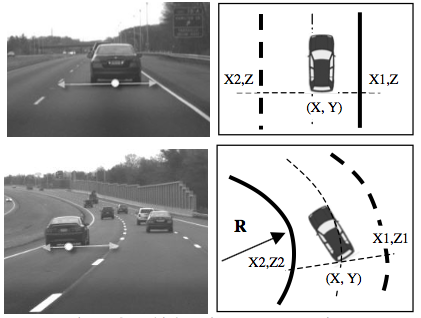
\includegraphics[scale=0.4]{figures/research_paper_figures/trajectory_multi-cue}
		\caption{Vehicle trajectory computation at straight and curved lanes \citep{multi-cue} }
		\label{fig:traj_multi-cue_image1}
	\end{minipage}\hfill
	\begin{minipage}{0.49\textwidth}
		\centering
		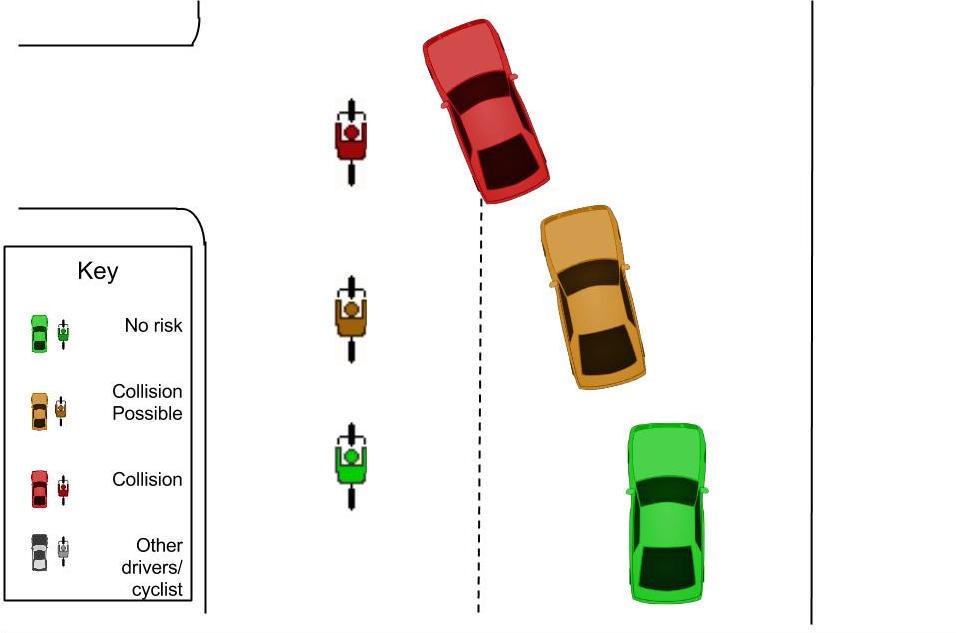
\includegraphics[scale=0.2]{figures/collision_avoidance_figures/Vehicle_changing_lane_into_the_path_of_a_cyclist}
		\caption{Cyclist and vehicle lane changing collision}
		\label{fig:change_lane_image}
	\end{minipage}
\end{figure}

\subsubsection{Learning Multi-Lane Trajectories using Vehicle-Based Vision \citep{multi-lane_traj}}



Conclusion - decision complying with criteria at the start

\subsubsection{Vehicle Trajectory Prediction}

\subsubsection{Bicycle Evasive Action}

\chapter{Prototype Analysis}
We created prototypes of the UI and of the bike hardware 
\section{Prototype 1}

\section{Prototype 2}

\chapter{User Interface Design}
\section{Overview of User Interface}  
\section{Screen Images}
\section{Screen Objects and Actions}

\chapter{Detailed Design}

\chapter{Conclusion}

\bibliographystyle{plainnat}
\bibliography{bibliography}

\end{document}          
